%%%%%%%%%%%%%%%%%%%%%%%%%%%%%%%%%%%%%
%
% CHECKLIST/TODO:
% - From reviewer: Please revise the abstract by some numerical findings as well.
% - Figure 1, add wall layers info and improve graphics
%
%%%%%%%%%%%%%%%%%%%%%%%%%%%%%%%%%%%%%%



%Fonts are typically available only in certain sizes/increments. As an example, the basic article document class loads only the following sizes (from size10.clo):

 %   \tiny @ 5pt;
 %   \scriptsize @ 7pt;
 %   \footnotesize @ 8pt;
 %   \small @ 9pt;
 %   \normalsize @ 10pt;
 %  \large @ 12pt;
 %   \Large @ 14.4pt;
 %   \LARGE @ 17.28pt;
 %   \huge @ 20.74pt; and
 %   \Huge @ 24.88pt


%%%%%%%%%%%%%%%%%%%%%%%%%%%%%%%%%%%%%%%%%%

\documentclass[10pt]{extarticle} %extendend font dimensions
\usepackage[margin=2cm,top=1cm,bottom=2cm]{geometry}
%\usepackage{helvet}
%\renewcommand{\familydefault}{\sfdefault}

%\usepackage[pass,showframe]{geometry}
\usepackage{amsmath}
\usepackage[english]{babel}

% author year bibliography  
\usepackage{natbib}
%\bibliographystyle{vancouver}
%\bibliographystyle{plainnat}
\bibliographystyle{agsm}
\renewcommand\harvardyearleft{\unskip, }
\renewcommand\harvardyearright[1]{.}

% Use of [T1]{fontenc}
% If you don't use \usepackage[T1]{fontenc}:
% - Words containing accented characters cannot be automatically hyphenated,
% - You cannot properly copy-and-paste such words from the output (DVI/PS/PDF),
% - Characters like the pipe sign, less than and greater sign give unexpected results.
\usepackage[T1]{fontenc}

\usepackage{newtxtext,newtxmath}

%%%%%%%%%% image packages:

\usepackage{graphicx}

\usepackage[export]{adjustbox}

\usepackage{subcaption}


%%%%%%%%%%%%%%%%%%%%%%%%%%

\renewcommand{\sfdefault}{phv} %makes arial the default font for sff

\newcommand{\bigsize}{\fontsize{12pt}{16pt}\selectfont} %12pt dim/ 16pt spacing

\newcommand{\subsecsize}{\fontsize{10pt}{10pt}\selectfont} %14pt dim 

\newcommand{\namesize}{\fontsize{10pt}{10pt}\selectfont} %13pt dim 

\usepackage[sf,pagestyles]{titlesec} % make section headings \sffamily

% headings formats:

\titleformat{\section}[block]
            {\sffamily\normalsize\bfseries}
            {\thesection.}{6pt}{\filright}
            
\titleformat{\subsection}[block]
            {\sffamily\subsecsize\bfseries}
            {\thesubsection.}{6pt}{\filright}

\titleformat{\subsubsection}[block]
            {\sffamily\subsubsecsize\bfseries}
            {\thesubsubsection.}{6pt}{\filright}

%% https://tex.stackexchange.com/questions/326331/titleformat-problem


%% Roman section numbering:
\renewcommand{\thesection}{\Roman{section}} 
\renewcommand{\thesubsection}{\thesection.\Roman{subsection}}

%% Fig. instead of Figure in figure captions:
\addto\captionsenglish{\renewcommand{\figurename}{Fig.}}

%title format:-----------------------
\usepackage{titling} % make titling elements \sffamily
\pretitle{\begin{center}\sffamily\bigsize\textbf}
\preauthor{\begin{center}
            \small\sffamily\ \lineskip 0.5em%
            \begin{tabular}[t]{c}}
%------------------------------------

% abstract format:-------------------
\usepackage{abstract}
% make abstract title \sffamily

\renewcommand\abstractnamefont{\sffamily\normalsize\bfseries}
\renewcommand{\abstracttextfont}{\sffamily\normalsize}
\renewcommand{\absnamepos}{raggedleft}
\setlength{\absleftindent}{0cm}
\setlength{\absrightindent}{0cm}

% ------------------------------------



\title{Comfort as the dead state of buildings: a preliminary discussion.}
\author{Valentina Bonetti\\ University of Strathclyde, Department of Mechanical and Aerospace Engineering, 75 Montrose St, Glasgow, G1 1XJ,  UK\\ \\ E-mail: valentina.bonetti@strath.ac.uk}

\date{}


\begin{document}
\renewcommand{\abstractname}{Abstract:}



\begin{figure}[!h]
\centering

\includegraphics[width=6.8in, center]{images/articleHeading1.png}
\end{figure}

%\maketitle
\let\newpage\relax
\vspace*{-2cm}
\maketitle
\vspace*{-1cm}


\begin{abstract}

\noindent Exergy is typically defined as the maximum work that can be extracted from a system when reaching equilibrium with its ``reference environment'' - a large region unaffected by the interactions - and derives from Gibbs' original concept of ``available energy of a body and medium''. The reference environment definition  plays a key role in exergy analysis but is still controversial, especially in the case of buildings; the most popular choice is the local outdoor air, because readily available and largely unaffected by the presence of the building, but its fluctuating conditions pose various challenges. The controversy around the reference environment arguably remains one of the main blockers in the practical application of building exergy methods.
However, going back to the origins, Gibbs defined available energy not only for a ``body and medium'', but also for the case of a ``body alone'', a system formed by subsystems in non-equilibrium conditions. Later, exergy too was defined for this second case, as the subsystem contribution to the body available energy. In the case of the ``body alone'', the reference is the ``dead state'' (or ``thermostatic state" of the body), in place of the reference environment. 
The main idea of this article is that building exergy analysis can be based not only, as currently, on the exergy definion originated by Gibbs' case of the ``body and medium'', but alternatively on the exergy definition originated by the case of the  ``body alone'', for which a large environment is not needed.  The outdoor reference environment can thus be substituted by an indoor ``dead state''. 
The study discusses possible system boundaries and ways of defining the building dead state based on indoor conditions, and the potential impact on building exergy analysis. The dynamic exergy modelling of a few cases is presented to visualise the numerical implications.

\end{abstract}

\noindent {\sffamily\normalsize\bfseries Keywords:}
{\sffamily\normalsize Exergy, reference environment, dynamic analysis.}


\section{Introduction} 

\sffamily\normalsize

%The problem
Building exergy analysis is an interesting concept, but it is hardly applied or even known in practice. The controversy on the reference state definition, the complexity of the analysis and the lack of convincing practical benefits are possibly the biggest obstacles to its utilisation. In the author's opinion, the main problem is the adoption of the varying outdoor air conditions as the reference state. First of all, outdoor fluctuations, combined with the inertia of the building envelope, make the outdoor environment not directly available; secondly, the meaning of ``warm" and ``cool" exergies based on the variable outdoor temperature can be misleading, especially because they are often treated as if they were always usable for heating and cooling. For instance in \cite{Choi2020} (left of page 11), energy stored at 25$^\circ C$ when the outdoor air is at 30$^\circ C$ is proposed as cool exergy useful for indoor cooling, and energy stored at 15$^\circ C$ when the outdoor air is at 10$^\circ C$ is considered as warm exergy that could be used for indoor heating, in a case where the indoor temperature is 20$^\circ C$; this is misleading because defining energy ``warm" or ``cool" because it is less cold or less hot than the outdoor air does not necessarily make it useful for heating or cooling purposes, but at most for fresh air pretreatment. As already observed in \cite{Bonetti2017a} (where some of the benefits of an exergy reference based on indoor comfort are discussed), defining warm and cool exergies on the base of outdoor variable conditions is not compatible with the common meaning of ``warm" and ``cold" and cannot be directly translated into heating or cooling.

% The idea
One alternative to variable outdoor air conditions is the use of indoor conditions. In the past, indoor air has been considered as a reference state for building exergy analysis, and the main argument against its use has been the fact that indoor air is not a large environment, as required by the definition of exergy \citep{Schmidt2011}. But where did this requirement come from? Answering this question requires going back to the origins.

% Gibbs (following line should be \citep{Klein1990} , but there is no space)
\cite{Gibbs1873} was the first to incorporate the first and second law of thermodynamics in one equation, in his paper "Graphical Methods in the Thermodyna\-mics of Fluids".  The combination of the first and second law led Gibbs to introduce the concept of ``available energy"; he distinguished two cases: a "body alone", in internal non-equilibrium conditions, and a "body and medium", in non-equilibrium conditions with each other. 

In the case of the ``body alone", the available energy of the body is the greatest amount of mechanical work that ideally can be obtained by taking the body, without any net contributions of energy from external objects, from the initial non-equilibrium condition to its point of stable or neutral equilibrium (on its ``surface of dissipated energy") that has the same entropy and volume of the initial state. The internal non-equilibrium state of the body can assume various forms, like a difference in the pressure of some of its part, or a gradient in temperature, or even different chemical compositions. It is important to observe that the term ``body" refers not necessarily to a single entity but to a system that is potentially including several subsystems and processes \citep{Gaggioli2012}.
In the case of the ``body and medium", the medium is supposed to be at uniform pressure and temperature and it is defined as ``reference environment": a large subsystem that is not affected by the interactions with the other components of the overall system, and is represented by a plane in Gibbs' energy-entropy-volume space. The available energy in this case is the distance (on the energy axis) from the point corresponding to the initial conditions of the body to the point with the same entropy and volume on the reference plane. Even if the body is in internal equilibrium, the combination between body and medium can still have available energy, unless they are in the same conditions. 


%Gaggioli
The vast majority of exergy analysis is based on the second case, the  ``body and medium", and relies on the definition of a reference environment (the medium). However, \cite{Gaggioli2012} examined in depth the meaning of ``dead state" and highlighted that exergy can be based on Gibbs' ``available energy of a body" (the first case mentioned above), which does not require a reference environment. The exergy of each subsystem of an overall system (in which no large one is required) was defined by \cite{Gaggioli1998} as the subsystem contribution to the available energy of the overall system, with the reference being the overall system ``dead state" - its ``thermostatic" conditions, where all the sub-parts are in equilibrium, subject to the given constraints. Such subsystem exergy is additive, and exergy balances can be used to perform exergy analysis. According to \cite{Gaggioli2012}, If subsystems are free to exchange entropy $S$ and volume $V$, the exergy content $Ex_i$ of each subsystem $i$ is $Ex_i = E + p_f - T_fS$, where the subscript $f$ indicates the dead state.

The main idea of this study is that building exergy analysis can be based on Gibbs' case of the ``body alone" and does not require a large environment, but can rather use, as the reference state, a definition of dead state related to indoor comfort. In order to make the ``body alone" relevant to building design, its boundaries include the indoor air and all the inner parts of the envelope that have a direct impact on indoor conditions (in practice, the depth of thermal mass that effectively contributes to the envelope interior storage). The dead state here proposed as a reference is a fixed ``target comfort" state, in order to avoid all the problems linked to reference fluctuation described by \cite{Pons2019}. This choice would make the definition of ``warm" and ``cool" exergies more straightforward to understand and relevant to heating and cooling strategies. The article discusses how different the proposed model is from Gibbs' case of the ``body alone", how distant the actual dead state of such system could be from a fixed comfort target, and what impact the discrepancies could have on exergy design and control strategies based on this reference.


\section{The dead state of a ``box" building} \label{subsec:simple}

Gibbs' ``body alone" was a closed and isolated system (although Gaggioli mentioned the possibility of having an open system \citep{Gaggioli1961}, where the dead state might vary). The closest real system which could be considered closed and isolated is a building with external high insulation, no openings and no internal loads, like the one in Fig. \ref{fig:esprmodel}, modelled with ESP-r for the UK climate. The outdoor has very low impact on its indoor conditions: considering system boundaries that include the envelope inner layers and the indoor air, thermostatic conditions (that can adopted as ``dead state") are reached after a short heating intervention, and freely maintained very stable for a long time (4 weeks are represented in Fig. \ref{fig:constructionelements}). Model and data are available at \cite{Bonetti2020}.

 
\begin{figure}[h]

\begin{subfigure}{0.35\textwidth}
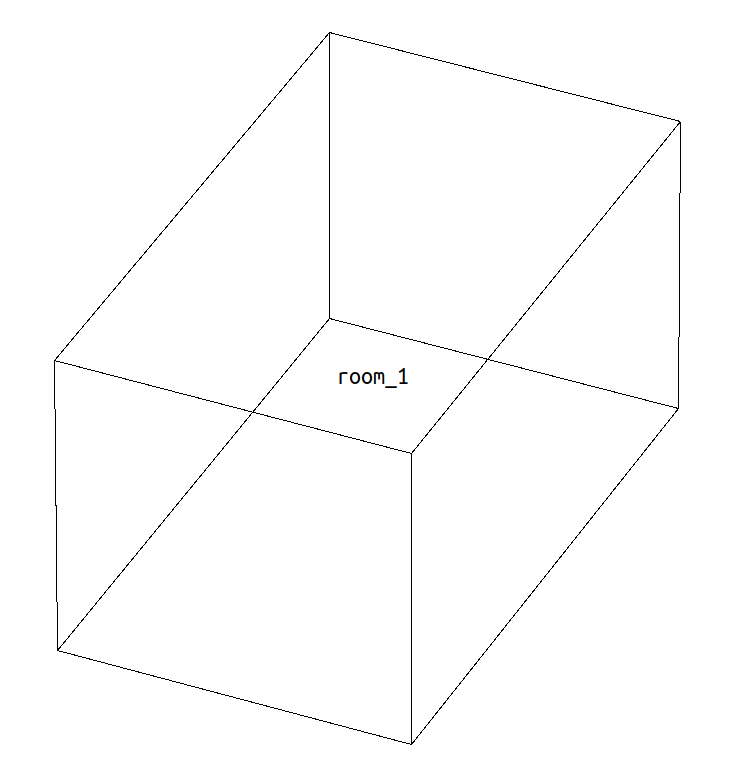
\includegraphics[width=0.95\linewidth, height=5.5cm]{images/Dead02_boxModel.png} 
\caption{ESP-r box model in a UK climate.}
\label{fig:esprmodel}
\end{subfigure}
\begin{subfigure}{0.65\textwidth}
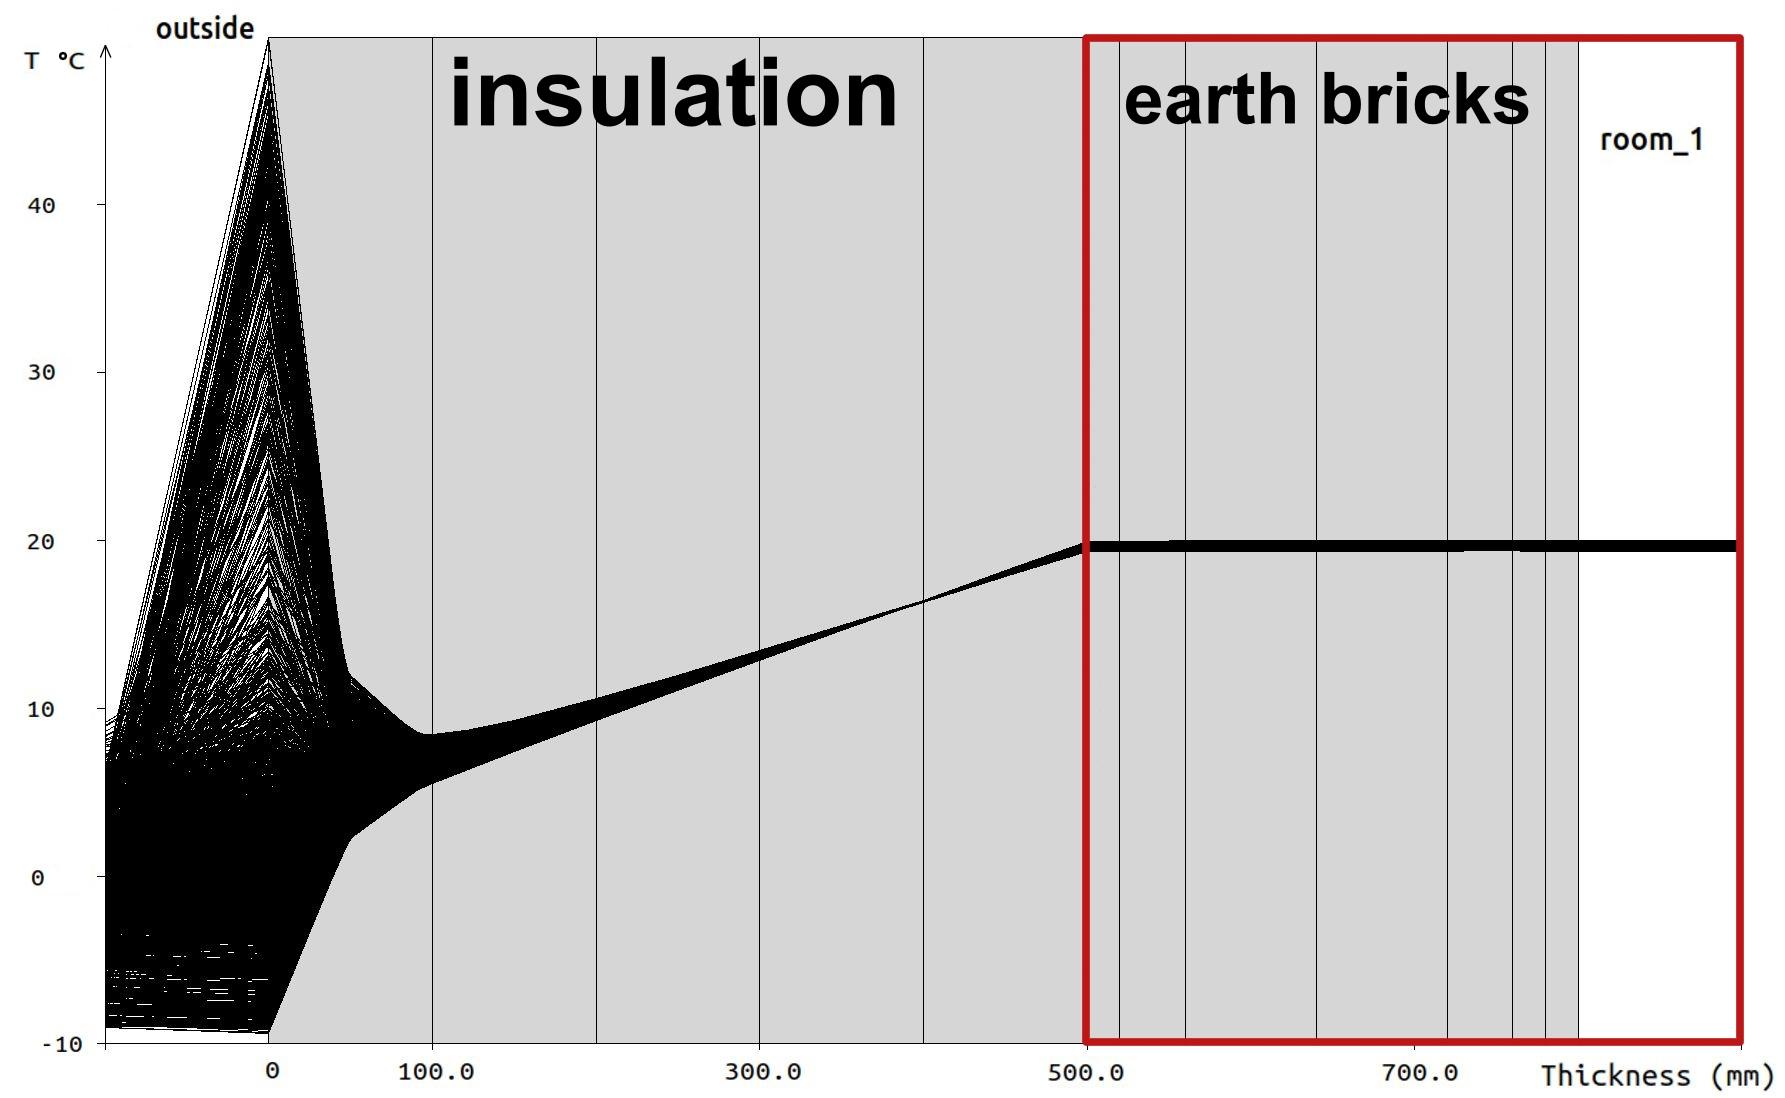
\includegraphics[width=0.95\linewidth, height=5.5cm]{images/01Feb_28Feb_Wall1_dead02_krita.jpg}
\caption{Cumulative values of intra-construction temperatures in a wall of the box model.}
\label{fig:constructionelements}
\end{subfigure}

\caption{The first case study: a box model with 500 mm of high  insulation and 300 mm of earth on the internal layers.}
\label{fig:casestudy}
\end{figure}





\section{The thermostatic state of realistic cases} \label{subsec:moreComplex}

Real buildings, especially in case of low performances, are not closed and isolated because of transmission losses, internal loads, solar gains, air exchanges. Consequently, the system constituted by the inner envelope layers and indoor air has a variable thermostatic state (the point at which all the subsystems are in equilibrium). However, the internal variations are much more limited than the outdoor air fluctuation, particularly for good envelopes; it is interesting to calculate the thermostatic state of real buildings for different zones and control strategies. 

In this brief article, the case in Fig. \ref{fig:casestudy} is considered sufficient to illustrate the point (model and data available from \cite{Bonetti2020}). The system boundaries are defined through an approximate estimate of ``periodic penetration depth" of 10 cm (or less, if an insulation layer is encountered) as suggested by the Standard DIN 4108. Different control strategies impact significantly. The thermostatic temperature $T_{eq}$ comes from the system energy balance: 

$T_{eq}(t)={\sum_i m_i c_i T_i(t)} / {\sum_i m_i c_i}$  \quad  (where $i$ = subsystem, $m$ = mass, $c$ = specific heat, $t$ = hourly timestep).

\vskip-0.35cm


\begin{figure}[h]
 
\begin{subfigure}{0.5\textwidth}
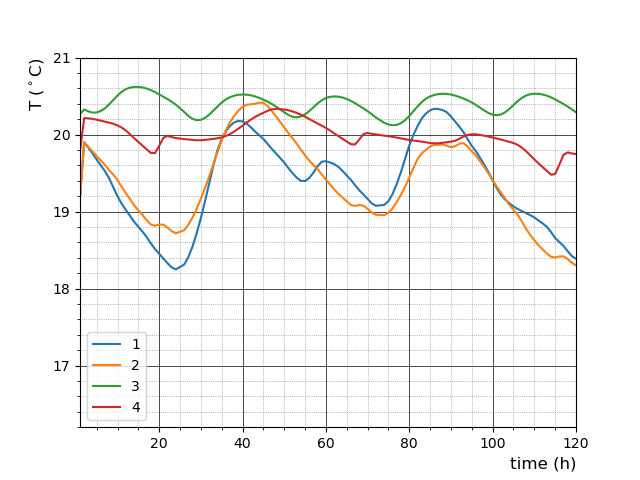
\includegraphics[width=0.99\linewidth, height=7cm]{images/1.png}
\vskip-0.1cm 
\caption{Radiant wall heating, set-point 21$^\circ C$ at night-time (9pm-6am)}
\label{fig:esprmodel}
\end{subfigure}
\begin{subfigure}{0.5\textwidth}
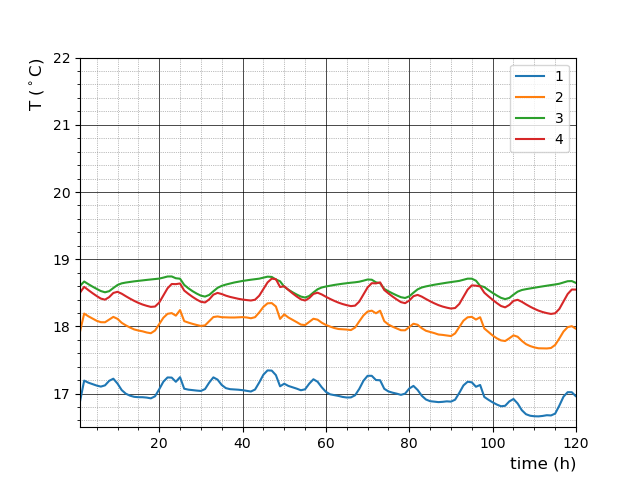
\includegraphics[width=0.99\linewidth, height=7cm]{images/2.png}
\vskip-0.1cm 
\caption{Basic air ideal heating, set-point 22$^\circ C$ (6am-8am + 6pm-10pm)}
\label{fig:constructionelements}
\end{subfigure}
 \vskip-0.2cm
\caption{The thermostatic temperature of 4 different thermal zones of a realistic model (5-day period in February, UK climate).}
\label{fig:casestudy}
\end{figure}

\section{Thermal exergy sensitivity} \label{sec:sensitivity}

\cite{Rosen2004} introduced the sensitivity $\sigma$, a measure of how exergy is impacted by variations in the reference state. In the case of thermal exergy, if heat $Q$ is exchanged at $T$ with a reference $T_0$ that varies by $\Delta T_0$: 


\vskip-0.1cm
\begin{equation}
\sigma =  {Ex(T_0+\Delta T_0)-Ex(T_0) \over Ex(T_0)} = { { Q \left( 1-{T_0+ \Delta T_0 \over T} \right) } - { Q \left( 1-{T_0 \over T} \right) } \over { Q \left( 1-{T_0 \over T} \right) } } = { \Delta T_0 \over T_0 - T }
\end{equation}

\vskip-0.2cm
\begin{figure}[h!]
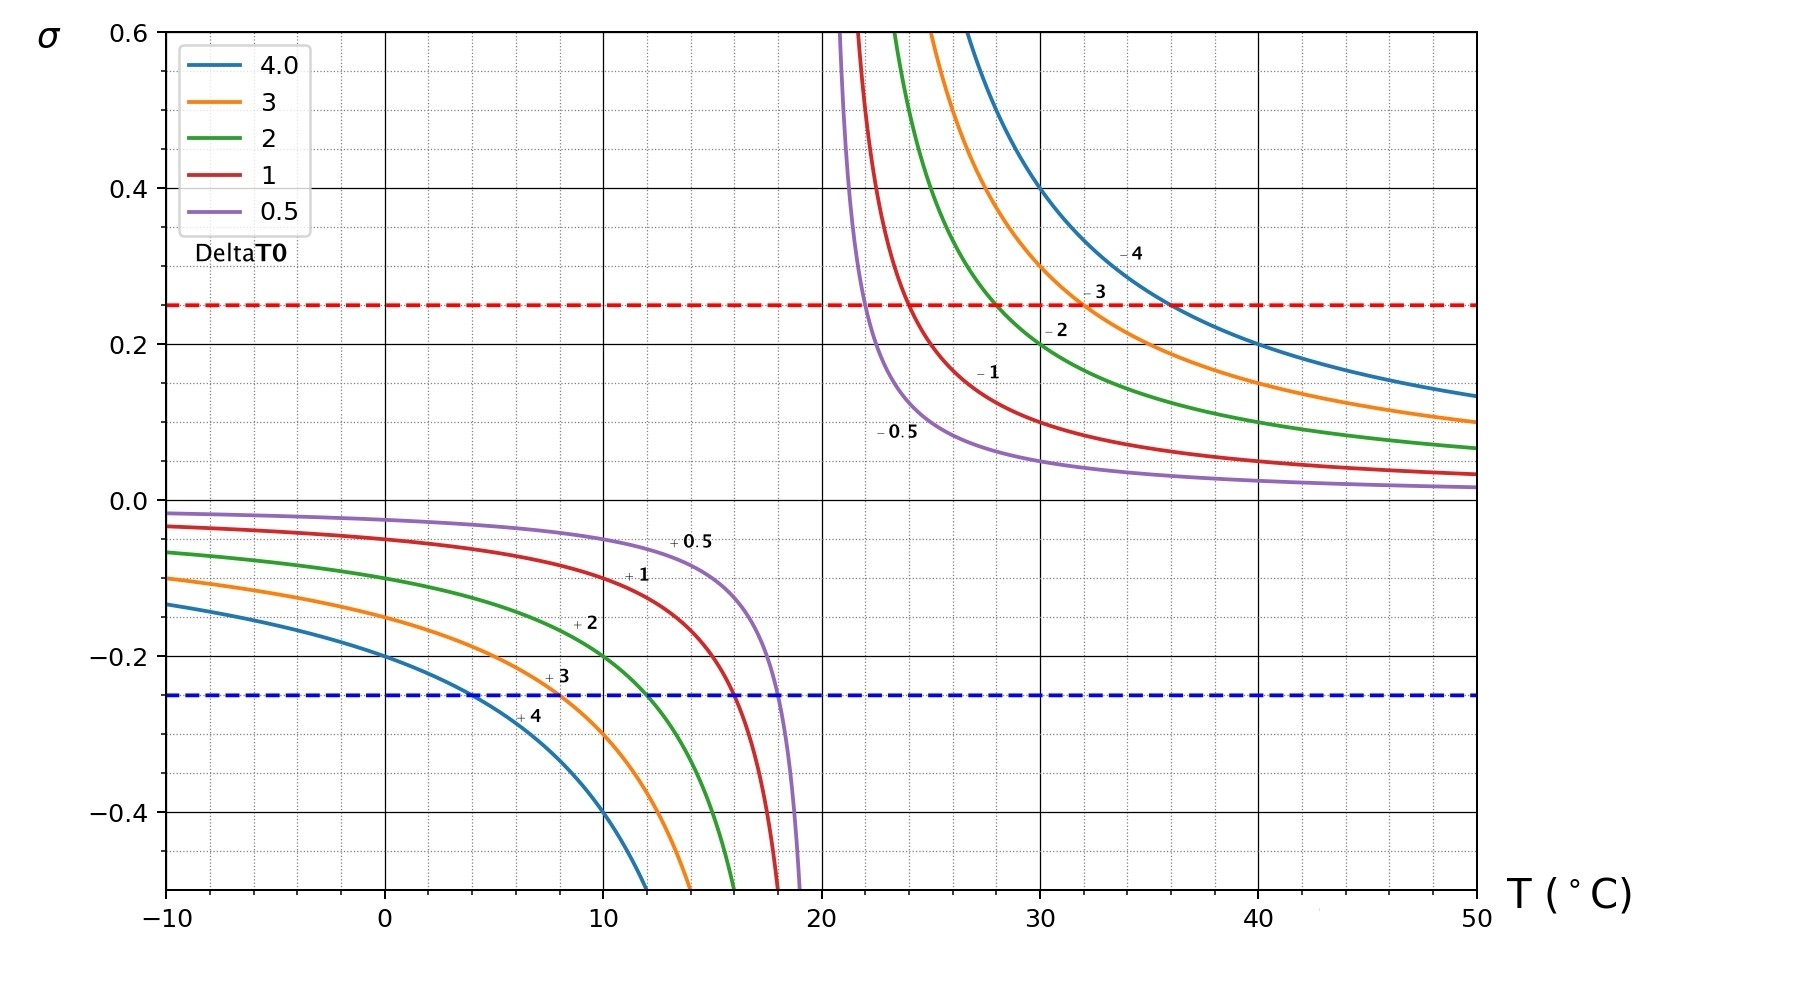
\includegraphics[height=6.2cm, center]{images/sensitivity_2.jpg} 
\caption{Thermal exergy sensitivity $\sigma$ against heat temperature $T$, for $T_0 = 20^\circ C$ and different reference variations $\Delta T_0$.}
\label{fig:sensitivity}
\end{figure}

\vfill \break


\noindent Fig. \ref{fig:sensitivity} shows that, if the reference temperatures variation remains within $\pm 0.5^\circ C$, exergy values are fairly accurate even for temperatures quite close to the reference ($\pm 10 \%$ around $15^\circ C$ and $25^\circ C$). For relatively large variations ($\pm 4^\circ C$), only exergies at temperatures under $4^\circ C$ or over $36^\circ C$ remain reasonably accurate ($\pm 25 \%$). The acceptance criteria depends on the aim of the analysis and should be investigated more in depth case by case. 
%%%%%%%%%%%%%%%

\section{Discussion: dead state and comfort targets} 

In most buildings the indoor environment, including the inner layers of the envelope, is in relatively stable conditions, dictated by comfort targets and control strategies. As soon as the temperature falls out of an acceptable range, the HVAC system intervenes to bring the conditions back to the desired value. If we define an overall system with boundaries that include the inner part of the envelope, the HVAC distribution (e.g. radiators) and the indoor and fresh air, its subsystems change dynamically to adapt to loads and chase the desired comfort. Although the thermostatic state of such a system is fluctuating, its conditions are generally fairly close to the comfort target, and adding all the internal loads and fluxes takes them even closer. We could then define a fixed dead state equal to the comfort requirements and obtain exergy values that are easy to calculate and interpret, and not far from the instantaneous reality of the indoor ambient (and thus relatively accurate, as discussed in section \ref{sec:sensitivity}). An in-depth discussion of why the exergy reference state should be fixed has been already presented by \cite{Pons2019}. It could be useful to consider whether the building exergy dead (or reference) state would be better defined through a fuzzy logic, to reflect the intrinsic nature of comfort as a range rather than a single value.



\section{Conclusions and future work}

The main idea of this article is that building exergy analysis can be based on a fixed reference equal to the target indoor comfort conditions - a sort of ``design dead state" of the indoor environment. The theoretical justification of this choice comes from the fact that exergy does not need a large reference environment to be defined, but can instead be based on the Gibbs' case of the ``body alone". Some advantages of this selection, focus of past and future work, are an easier and clearer analysis - the meaning of ``warm" and ``cold" exergy now coincides with the common meaning of ``warm" and ``cold" - and a shifted attention to the energy quality of the indoor ambient, which could for instance facilitate the design of demand-offer decoupling strategies.


\section*{Acknowledgements}

The author thanks the Engineering and Physical Sciences Research Council U.K. (EPSRC, Grant No.1586601) and the Building Research Establishment (BRE) for the past financial support.

{\small %font size 9
 \bibliography{ValeIEEES2020}
}
%% Max 10-15 refs
% NOTES FOR BIBLIOGRAPHY
% References“Arial, 10 points, bold”
% “Arial, 9 points, alphabetic order of names (first author), max 10-15 important references.”
% “If Mendeley is used, you can select Journal of Cleaner Production or similar referencing styles”

\vfill \break



\end{document}




% LaTeX references:

% Use of package [T1]{fontenc}: 
% https://tex.stackexchange.com/questions/664/why-should-i-use-usepackaget1fontenc

% https://tex.stackexchange.com/questions/25249/how-do-i-use-a-particular-font-for-a-small-section-of-text-in-my-document

% abstract package documentation:
% http://citeseerx.ist.psu.edu/viewdoc/download?doi=10.1.1.169.8953&rep=rep1&type=pdf

% title formats using titlesec:
% http://mirror.ox.ac.uk/sites/ctan.org/macros/latex/contrib/titlesec/titlesec.pdf
% https://tex.stackexchange.com/questions/326331/titleformat-problem

